\section{Application Implementation}
This section will describe the implementation of the study application, mostly regarding how data was collected, how features were computed as well as how the data was sent to a Firebase instance. The study app used the package while it was in an earlier iteration. In this iteration almost none of the logic related to storing and loading data was part of the packagee, and as such all of this had to be written in the application instead.

\subsection{Component Overview}
To provide a high level overview of the different components which make up the study application a component diagram displayed in Figure \ref{fig:app-component-diagram}. The MobilityStudy component in blue is the component responsible for managing the application state but does not do much outside of this since the application state management required is minimal. Had it been a more complex application with many different screens and a state which had to be maintained across these screens (for example a shopping cart in a shopping app) then more logic would lie inside the MobilityStudy component. Instead the Main Screen is spawned from the MobilityStudy component which in turn creates an AppProcessor instance. The AppProcessor instance is responsible for a multitude of tasks, such as asking for permissions, collection location data, and computing features. Storing and loading from the disk is done through the FileManager component which includes location data, Stops, Moves, MobilityContexts and diary answers. This component is also responsible for uploading the stored data to Firebase.

\begin{figure}
    \centering
    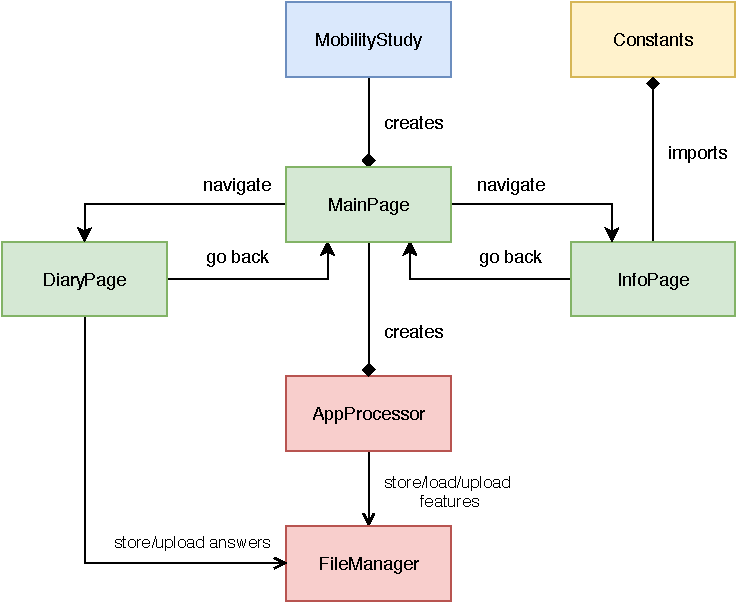
\includegraphics[width=\textwidth]{images/diagrams/app-diagram.pdf}
    \caption{Component diagram for the study application displaying the different building blocks and the interactions between them}
    \label{fig:app-component-diagram}
\end{figure}
